\chapter{Clasificación de superficies compactas}

\section{Símplices}

\defn{Símplice}{
    Dados $k+1$ puntos $v_0,\dots,v_k\in\R^m$ afínmente independientes, el subconjunto convexo de $\R^m$ más pequeño que los contiene se conoce como un k-símplice y se denota por $\sigma = [v_0, \dots, v_k]$. Los puntos $v_i$ se llaman los vértices del k-símplice. Diremos que la dimensión de $\sigma$ es $k$.
}
\defn{Subsímplices, caras}{
    Si $\sigma=[v_0,\dots,v_k]$ es un k-símplice, cualquier subconjunto no vacío de vértices tambien determina un símplice que llamaremos subsímplice de $\sigma$. Si solo se omite un vértice, el subsímplice correspondiente se denomina una cara.
    \[\text{Las caras de }\sigma\text{ se denotan: } [v_0, \dots, \hat{v}_i, \dots, v_k], \text{ donde } \hat{v}_i \text{ es el vértice omitido.}\]
}

\ex{
    0-símplice (punto), 1-símplice (segmento de línea), 2-símplice (triángulo) y 3-símplice (tetraedro)
    \begin{center}
        \includegraphics[width=0.7\linewidth]{img/ejemplos-simplices.png}
    \end{center}
}

\defn{Frontera}{
    Si $\sigma=[v_0,\dots,v_k]$ es un k-símplice, la unión de todas sus caras se denomina la frontera de $\sigma$ y se denota por 
    \[\partial\sigma = \displaystyle \bigcup_{0 \le i \le k}[v_0, \dots, \hat{v}_i, \dots, v_k].\]
}
\defn{Interior}{
    Si $\sigma$ es un k-símplice, el complementario de su frontera se denomina el interior de $\sigma$, 
    \[\text{int}(\sigma) = \sigma \setminus \partial\sigma\]
    Inmediatamente, se obtiene $\sigma = \text{int}(\sigma) \cup \partial\sigma$, donde la unión es disjunta.
}

\rmkb{
    La frontera y el interior de un k-símplice \(\sigma\) son conceptos independientes de la topología tomada sobre \(\R^m\). Sin embargo, si \(k = m\), entonces coinciden con la frontera y el interior topológicos de \(\sigma\) en topología usual de \(\R^m\).
}

\section{Complejos simpliciales}

\defn{Complejo simplicial}{
    Un complejo simplicial $K$ es una colección finita de símplices tal que:
    \begin{enumerate}
        \item Cada cara de cada símplice de $K$ también está en $K$.
        \item La intersección de cualesquiera dos símplices de $K$ es vacía o es un subsímplice de ambos.
    \end{enumerate}
    La dimensión de $K$ es la máxima dimensión de sus símplices.
}
\defn{Número de Euler}{
    Sea $K$ un complejo simplicial de dimensión n, si para cada $0 \le k \le n$ denotamos por $i_k$ el número de k-símplices de $K$, entonces el número (o característica) de Euler de $K$ es:
    \[\chi (K) = i_0 - i_1 + \dots + (-1)^n i_n.\]
}
\rmkb{
    Para el caso de un complejo simplicial de dimensión 2, denotando a los vértices $V = i_0$, aristas (edges en inglés) $E = i_1$ y caras (faces en inglés) $F=i_2$; la característica de Euler se puede expresar como:
    \[\chi = V - E + F\]
    
}
\defn{Poliedro asociado}{
    Dado un complejo simplicial $K$, la unión de todos los símplices de $K$ con la topología inducida por la topología usual de $\R^n$ se denomina el poliedro de $K$ y lo denotamos por $|K|$.
}

\section{Triangulaciones}

\defn{Triangulación}{
    Una triangulación de dimensión $n$ de un espacio topológico $X$ es un complejo simplicial $K$ de dimensión $n$ de forma que $|K|$ y $X$ son homeomorfos. En este caso se dice que $X$ es triangulable.
}

Enunciamos el siguiente teorema sin demostración:

\thmr{Teorema de Radó}{rado}{
    Toda superficie topológica admite una triangulación por un complejo simplicial de dimensión 2. Además cada 1-símplice (arista) es subsímplice de exactamente dos 2-símplices (cara).
}

\section{Presentación de superficies}

\defn{Letras y palabras}{
    Sea $A$ un conjunto finito (sus elementos los llamaremos letras). Una palabra $W$ es una sucesión finita de elementos de la forma $a$ ó $a^{-1}$, con $a \in A$, denotada por yuxtaposición.
}

\ex{
    Consideremos el conjunto $A=\{a,b,c\}$ formado por tres letras. Algunos ejemplos de palabras son los siguientes:
    \[W_1=cbab^{-1}ca^{-1},W_2=caab^{-1}bc^{-1},W_3=abb^{-1}a^{-1}.\]
}

\defn{Presentación poligonal}{
    Una presentación poligonal, escrita como $\partes =\langle A|W_1,\dots,W_k\rangle$, está formada por un conjunto finito de letras $A$ y una colección finita de palabras $W_1,\dots,W_k$ que cumplen:
    \begin{enumerate}
        \item Cada letra de $A$ aparece exactamente dos veces en todo el conjunto de palabras.
        \item Cada palabra tiene al menos longitud tres, salvo que haya una sola palabra que podría ser de dos letras.
    \end{enumerate}
}

\ex{
    Algunos ejemplos sencillos de presentaciones poligonales son los siguientes:
    \[\partes_1=\langle a\mid  aa^{-1}\rangle, \partes_2=\langle a,b\mid  aba^{-1}b^{-1}\rangle.\]

    \noindent Si consideramos el conjunto de letras y palabras del ejemplo anterior, $\partes=\langle A \mid W_1 \rangle$ es una representación poligonal, pero $\partes'=\langle A \mid W_3 \rangle$ no, ya que la letra $c$ no aparece exactamente dos veces en el conjunto de palabras.
}

\defn{Realización geométrica de $\partes$}{
    Toda presentación poligonal $\partes$ tiene asociado un espacio topológico $|\partes|$ (realización geométrica de $\partes$) construido como sigue: 
    \begin{enumerate}
        \item Para cada palabra se considera un polígono con el mismo número de aristas que la longitud de la palabra. 
        \item Cada arista se etiqueta correlativamente con las letras de la palabra y orientación opuesta si la letra está elevada a -1. 
        \item Finalmente, se identifican las aristas con el mismo nombre y orientación, mediante la topología cociente.
    \end{enumerate}
}

\clearpage

\ex{
    Ejemplos de realizaciones geométricas y espacios a los que son homeomorfas:
    \begin{center}
        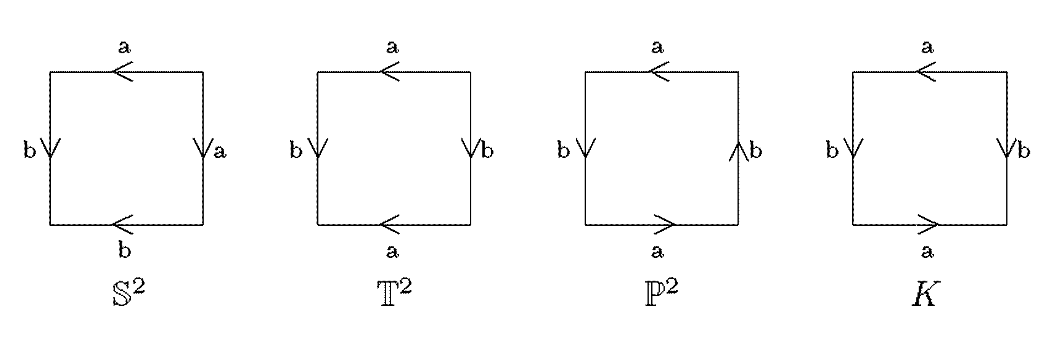
\includegraphics[width=0.9\textwidth]{img/realizacion-geom.png}
    \end{center}

    Si nos fijamos en la segunda realización geométrica, esta es claramente homeomorfa al cuadrado unidad $X=I \times I$ con la relación de equivalencia
    \[
        (x_1,y_1)\sim(x_2,y_2) \iff x_1-x_2\in\mathbb{Z}, y_1-y_2\in\mathbb{Z}
    \]
    que identifica los lados superior e inferior con la misma orientación y también derecho e izquierdo con la misma orientación. Este espacio cociente $\faktor{X}{\sim}$ es precisamente el que tratamos en un ejemplo de la Sección 1.2, donde se probó que era homeomorfo a $\mathbb{T}^2$.
}

\exer{
    Probar que las realizaciones geométricas del ejemplo anterior, es decir, los cuadrados con una cierta relación de equivalencia, son homeomorfos a los espacios que se indica en la figura.
}

\propp{Compacidad y conexión de $|\partes|$}{\label{prop:244}
    Dada una representación poligonal $\partes$, su realización geométrica, $|\partes|$, es una superficie compacta. Además si solo tiene una palabra, entonces es conexa.
}{
    Consideremos el polígono $X$ (realmente pueden ser varios polígonos disjuntos si hay más de una palabra). Vamos a ver que el espacio topológico cociente $\tilde{X}$ resultado de identificar las aristas es:
    \begin{enumerate}
        \item Compacto
        \item Superficie ($T_2$, $2A\N$, localmente euclídeo)
    \end{enumerate}

    Antes de esto, es inmediato que si hay una sola palabra el espacio es conexo, puesto que en tal caso el espacio original $X$ está formado por un único polígono y es conexo. Por tanto, por las propiedades de los espacios cociente $\tilde{X}$ también es conexo. Notemos también que el hecho de tener más de una palabra no excluye la posibilidad de que $\tilde{X}$ sea conexo.

    \textbf{Compacto:} Sea $X$ el polígono en $\R^2$, sea $\sim$ la relación de equivalencia entre las aristas y sea $\tilde{X}$ el cociente. $X$ es compacto por ser cerrado y acotado, y la proyección al cociente $p : X \to \tilde{X}=\faktor{X}{\sim}$  es continua, por tanto, $\tilde{X}$ es compacto.

    \textbf{$\mathbf{T_2}$:} \textit{Esquema de la demostración:}
    
    Consideremos dos puntos $x',y'\in\tilde{X}$ y sean $x,y\in X$ de tal manera que $p(x)=x',p(y)=y'$. Podemos tomar discos en $\R^2$ lo suficientemente pequeños de forma que separen los puntos en $X$ y las imágenes por $p$ separan los puntos de $\tilde{X}$.

    \textbf{Localmente euclídeo:} La idea es distinguir 3 casos: 

    Veamos que $\tilde{X}$ es localmente euclídeo. Necesitamos que para cada punto, haya un entorno que sea homeomorfo a un abierto de $\R^2$. 
    Sea $x \in \tilde{X}$ y consideramos los tres casos posibles para la preimagen del punto:
    \[
        \pi^{-1}(x) =
        \begin{cases}
            p \in \text{int}(X) \\
            \{q_1, q_2\} \in \text{aristas} \\
            \{v_1, \dots, v_k\} \in \text{vértices}
        \end{cases}
    \]
    \begin{enumerate}
        \item $\pi^{-1}(x) = p \in \text{int}(X)$. Como solo se identifican aristas estamos dentro de un polígono de $\R^2$. Entonces, $\pi|_{\text{int}(X)} : \text{int}(X) \to \pi(\text{int}(X))$ es biyectiva y continua y su inversa también es continua. Por tanto, como $\text{int}(X)$ es abierto, $\pi(\text{int}(X))$ es un entorno del $x$ homeomorfo a un abierto como queríamos ver.
        
        \item Tomamos $D_i \subset \R^2$ disco centrado en $q_i$ con $\overline{D_1} \cap \overline{D_2} = \emptyset$. Además, tampoco cortan ningun vértice de $X$.
        Sean $U_i = D_i \cap X$ semidiscos. Sea $h : a \to a'$ el homeomorfismo que da la relación de equivalencia (con $a, a'$ las aristas), es decir, $h(x)=y, x \in a, y \in a' \iff xRy$. 
        
        \begin{center}
            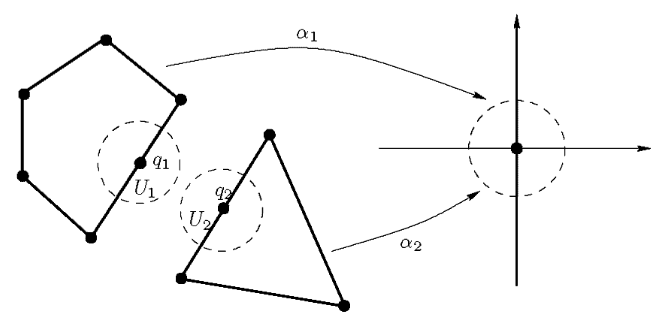
\includegraphics[width=0.8\textwidth]{img/entornos-aristas.png}
        \end{center}

        Existen homeomorfismos $\alpha_i : \R^2 \to \R^2$ (de hecho aplicaciones afines) tales que: 
        \begin{align*}
        \alpha_1(U_1) &= \{z\in \mathbb{C} : |z| < r_1, \text{Im}(z) \ge 0\} \equiv \{(x,y)\in\R^2 : \|(x,y)\| < r_1, y \ge 0\}\\
        \alpha_2(U_2) &= \{z\in \mathbb{C} : |z| < r_2, \text{Im}(z) \le 0\}
        \end{align*}
        que verifican que $\alpha_2 \circ h = \alpha_1|_a$ y que mandan $q_1,q_2$ al origen.
        
        Sea $r = \min\{r_1, r_2\}$ y definamos los abiertos
        \[
        V_1 = \alpha^{-1}(\{z : |z|<r, \text{Im}(z) \ge 0\}),\quad V_2 = \alpha^{-1}(\{z : |z|<r, \text{Im}(z) \le 0\})
        \]
        
        Consideremos ahora $V=V_1 \cup V_2$ abierto de $X$. Entonces $\alpha : V_1 \cup V_2 \to B(0,r)$ definida por 
        \[
        \alpha(x) = \begin{cases}
            \alpha_1(x) & x \in V_1 \\
            \alpha_2(x) & x \in V_2.
        \end{cases}
        \]
        es una identificación (continua, cerrada, sobreyectiva). Está bien definida y pasa al cociente porque $xRy, x\in a, y \in a' \implies y = h(x)$ y entonces $\alpha(y) = \alpha_2(y) = \alpha_2(h(x)) = \alpha_1(x) = \alpha(x)$. Al pasar al cociente obtenemos $\tilde{\alpha}:\tilde{V}\to\R^2$, donde $\tilde{V}=\pi(V)$ que es abierto, como $x\in\tilde{V}$ esto prueba que existe un entorno de $x$ homeomorfo a un entorno de $\R^2$, puesto que podemos consideramos la restricción de $\tilde{\alpha}$ a su imagen (que será abierta puesto que $\tilde{V}$ lo es), de manera que obtenemos un homeomorfismo.

        \item Sea ahora $\pi^{-1}(x) = \{v_1, \dots, v_k\}, k \in \N$. Consideremos $D_i$ discos suficientemente pequeños de manera que $\overline{D_i} \cap \overline{D_j} = \emptyset, i \neq j$ no contenga puntos de otras aristas, ni vértices. 
        Sean $U_i = D_i \cap X$ sectores circulares. Denotemos a las dos aristas de cada vértice $a_i,b_i$, y supongamos los sectores ordenados de forma que $b_i \sim a_{i+1}, i=1,\dots,k$.

        Objetivo: encontrar una aplicación que junte todos los sectores para formar una circunferencia, $V_1 \cup \dots \cup V_k \overset{\alpha}{\longrightarrow} B(0,r) \subset \R^2$. 
        
        \begin{center}
            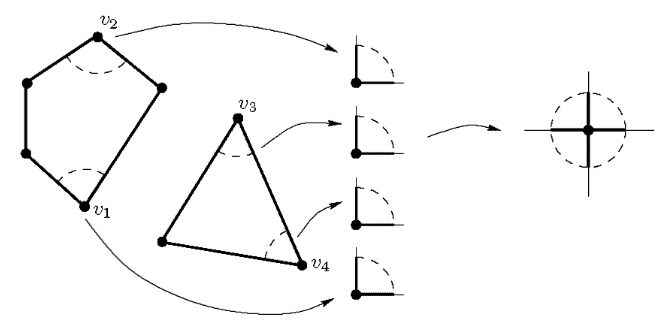
\includegraphics[width=0.8\textwidth]{img/entornos-vertices.png}
        \end{center}

        En primer lugar podemos construir un homeomorfismo afín $\alpha_i : \R^2 \to \R^2$ que lleva el sector $U_i$ en $\{z : |z| < r_i, \text{arg}(z) \in [\frac{2\pi(i-1)}{k}, \frac{2\pi i}{k}]\}$ para todo $i=1,\dots,k-1$ cumpliendo $\alpha_{i+1} \circ h_i = \alpha_i|_{b_i}$, donde $h_i : b_i \to a_{i+1}$.
        
        También podemos construir el último homeomorfismo $\alpha_k : \R^2 \to \R^2$ que lleva $U_k$ en $\{z : |z| < r_k, \text{arg}(z) \in [\frac{2\pi(k-1)}{k}, 2\pi]\}$ y que cumpla 
        \[
            \begin{cases}
                \alpha_k \circ h_{k-1} = \alpha_{k-1}|_{b_{k-1}} \\
                \alpha_1 \circ h_k = \alpha_k|_{b_k \equiv a_1} \tag{$\star$}
            \end{cases}
        \]
        con $h_k : b_k \to a_1$.
        
        Para garantizar la existencia de $\alpha_k$, podemos construirla en dos pasos, una para llevar a su hueco y otra para garantizar ($\star$). 

        Sea $r \le \min\{r_1, \dots, r_k\}$ y $V_i = \alpha_i^{-1}(\{z : |z| < r, \text{arg}(z) \in [\frac{2\pi(i-1)}{k}, \frac{2\pi i}{k}]\})$. Definimos $\alpha : V_1 \cup \dots \cup V_k \to B(0,r)$ como
        \[
        \alpha(x) = \alpha_i(x), x \in V_i.
        \]
        $\alpha$ está bien definida pues
        \[
        xRy, x\in b_i, y \in a_{i+1} \implies \alpha(y) = \alpha_{i+1}(h_i(x)) = \alpha_i(x) = \alpha(x), i\ne k.
        \]
        Y para $i=k$,
        \[
        y = h_k(x) \in a_1, \alpha(y)=\alpha_{1}(h_k(x))=\alpha_k(x)=\alpha(x).
        \]
        Luego, $\alpha$ es identificación (continua, sobreyectiva, cerrada) y $\tilde{\alpha}$ es un homeomorfismo al restringirla a su imagen, y podemos aplicar el mismo argumento del caso anterior.
    \end{enumerate}

    \textbf{$\mathbf{2A\N}$:} La proyección es continua y sobreyectiva, y el polígono es $2A\N$, luego $\tilde{X}$ también lo es por el \hyperref[lem:146]{Lema 1.4.6}.
}

\defn{Presentación de una superficie compacta}{
    Sea $\mathcal{S}$ una superficie compacta. Una presentación de $\mathcal{S}$ es una presentación poligonal $\partes$ tal que $|\partes|$ y $\mathcal{S}$ son homeomorfas.
}

\clearpage

\section{Transformaciones elementales}

\defn{Transformaciones elementales sobre presentaciones poligonales}{
    Dada una presentación poligonal, llamaremos transformaciones elementales a las siguientes operaciones:
    \begin{itemize}
        \item \textbf{Renombrado:} Sustituir todas las apariciones de una letra $a$ por otra letra $b$ que no estuviera en la presentación.
        \item \textbf{Subdivisión:} Cambiar todas las apariciones de una letra $a$ por $ab$, y todas las apariciones de $a^{-1}$ por $b^{-1}a^{-1}$, donde $b$ es una letra nueva que no estaba en la presentación.
        \item \textbf{Consolidado: } Dadas dos letras $a$ y $b$ que siempre aparezcan juntas de la forma $ab$ o $b^{-1}a^{-1}$, sustituimos todas las apariciones de $ab$ por $c$, y todas las apariciones de $b^{-1}a^{-1}$ por $c^{-1}$, donde $c$ es una letra nueva que no estaba en la presentación.
        \item \textbf{Reflejo: } Cambiar una palabra de la forma $a_1a_2\dots a_k$ por $a_k^{-1}a_{k-1}^{-1}\dots a_1^{-1}$, donde $a_i$ son letras de la presentación.
        \item \textbf{Rotación: } Cambiar una palabra de la forma $a_1a_2\dots a_k$ por $a_2a_3\dots a_k a_1$, donde $a_i$ son letras de la presentación.
        \item \textbf{Corte:} Dada una palabra $W_1W_2$, con $W_1$ y $W_2$ no vacías, quitamos $W_1W_2$ de la presentación y añadimos $W_1a, a^{-1}W_2$ como palabras nuevas, donde $a$ es una letra nueva que no estaba en la presentación.
        \item \textbf{Pegado} Sustituimos dos palabras de la forma $W_1a, a^{-1}W_2$, con $W_1$ y $W_2$ arbitrarias y no vacías, por $W_1W_2$.
        \item \textbf{Plegado} Una palabra de la forma $W_1aa^{-1}$ se sustituye por $W_1$, donde $W_1$ tiene al menos longitud 3, salvo que haya una sola palabra, en cuyo caso podría ser de dos letras.
        \item \textbf{Desplegado} Una palabra de la forma $W_1$ se sustituye por $W_1aa^{-1}$, donde $W_1$ tiene al menos longitud 3, salvo que haya una sola palabra, en cuyo caso podría ser de dos letras.
    \end{itemize}
}

\defn{Presentaciones equivalentes}{
    Dos transformaciones poligonales se dice que son topológicamente equivalentes si sus realizaciones geométricas son homeomorfas.
}

\propp{Equivalencia por transformaciones elementales}{
    Cada una de las transformaciones elementales sobre una presentación poligonal produce otra presentación topológicamente equivalente. 
}{
    Claramente, subdividir y consolidar son operaciones inversas una de la otra, al igual que cortar/pegar y plegar/desplegar, por lo que por simetría solo es necesario demostrar una de cada par. Demostramos las técnicas probando la proposición para cortar y plegar, y dejamos el resto como ejercicio.

    Para probar que cortar produce una realización geométrica homeomorfa, sean \(P_{1}\) y \(P_{2}\) polígonos convexos <<etiquetados>> \(W_{1}e\) y \(e^{-1}W_{2}\), respectivamente, y sea \(P^{\prime}\) un polígono convexo etiquetado \(W_{1}W_{2}\). Por el momento, asumamos que estas son las únicas palabras en sus respectivas presentaciones. Sean \(\pi: P_{1}\sqcup P_{2}\to S\) y \(\pi' P^{\prime}\to S^{\prime}\) las identificaciones respectivas. El segmento de recta que va desde el vértice terminal de \(W_{1}\) en \(P^{\prime}\) hasta su vértice inicial está contenido en \(P^{\prime}\) por convexidad; etiquetemos este segmento como \(e\). Se puede asegurar\footnote{Haría falta hacer una construcción que no incluimos, pero se puede probar que las aplicaciones que nombramos existen.} que existe una aplicación continua \(f: P_{1}\sqcup P_{2}\to P^{\prime}\) que lleva cada arista de \(P_{1}\) o \(P_{2}\) a la arista en \(P^{\prime}\) con la etiqueta correspondiente, y cuya restricción a cada \(P_{i}\) es un homeomorfismo. Además, \(f\) es una identificación. Como \(f\) identifica las dos aristas etiquetadas \(e\) y \(e^{-1}\) pero nada más, las también identificaciones \(\pi'\circ f\) y \(\pi\) realizan exactamente las mismas identificaciones, por lo que sus espacios cociente son homeomorfos. Si hay otras palabras \(W_{3},\ldots,W_{k}\), simplemente extendemos \(f\) declarándola como la identidad en sus respectivos polígonos y procedemos como antes.

    Para plegar, como antes podemos ignorar las palabras adicionales \(W_{2},\ldots,W_{k}\). Si \(W_{1}\) tiene longitud \(2\), podemos subdividir para alargarla, luego realizar la operación de plegado y después consolidar, así que asumimos que \(W_{1}\) tiene longitud al menos \(3\). Supongamos primero que \(W_{1}=abc\) tiene longitud exactamente \(3\). Sean \(P\) y \(P^{\prime}\) polígonos convexos con etiquetas de arista \(abcee^{-1}\) y \(abc\), respectivamente, y sean \(\pi\colon P\to S\), \(\pi^{\prime}\colon P^{\prime}\to S^{\prime}\) las identificaciones.
    \begin{center}
        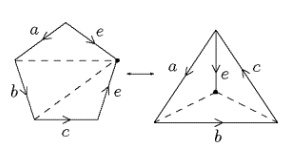
\includegraphics[width=0.3\textwidth]{img/plegado.png}
    \end{center}

    Añadiendo aristas como se muestra en la figura existe una única aplicación \(f: P\to P^{\prime}\) que lleva cada arista de \(P\) a la arista de \(P^{\prime}\) con la misma etiqueta. Como antes, \(\pi^{\prime}\circ f\) y \(\pi\) son identificaciones que realizan las mismas identificaciones, por lo que sus espacios cociente son homeomorfos.

    Si \(W_{1}\) tiene longitud \(4\) o más, podemos escribir \(W_{1}=Xbc\) para algún \(X\) de longitud al menos \(2\). Entonces cortamos a lo largo de \(a\) para obtener $\langle S,b,c,e \mid Xbcee^{-1}\rangle\cong\langle S,a,b,c,e \mid Xa^{-1},abcee^{-1}\rangle$
    y procedemos como antes.
}

\propp{Presentación de $\mathcal{S}_1\#\mathcal{S}_2$}{
    Sean $\mathcal{S}_1$ y $\mathcal{S}_2$ dos superficies compactas y conexas presentadas por $\langle A_1|W_1 \rangle$ y $\langle A_2|W_2 \rangle$, respectivamente. Entonces, $\langle A_1 \cup A_2|W_1W_2 \rangle$ es una presentación de $\mathcal{S}_1\#\mathcal{S}_2$.
}{
    Sea $\partes_1$ el polígono asociado a $W_1$ y sean $p,q \in \text{int}(\partes_1)$ dos puntos distintos y $v$ un vértice de $\partes_1$. 

    Aplicando operaciones elementales tenemos
    \[
    \mathcal{S}_1 = \langle A_1|W_1 \rangle = \langle A_1 \cup \{a,b,c\} \mid W_1cba = Q_1, a^{-1}b^{-1}c^{-1} \rangle.
    \]
    Definimos $\pi' : \partes_1 \cup Q_1 \to \mathcal{S}_1$ y $\pi:\partes_1 \to \mathcal{S}_1$. Sea entonces $B_1 = \pi'(\text{int}(Q_1)) \subset \mathcal{S}_1$. Si probamos que $B_1$ es homeomorfo a un disco, entonces podemos hacer lo mismo con $\mathcal{S}_2$ y aplicar que que $\mathcal{S}_1\#\mathcal{S}_2$ se puede ver como $\faktor{\mathcal{S}_1 \setminus Q_1 \sqcup \mathcal{S}_2\setminus Q_2}{R_\varphi}$.

    Para ver que $B_1$ es homeomorfo a un disco, hacemos un razonamiento similar al de la \hyperref[prop:244]{Proposición 2.4.4} tomando como abierto uno de la forma <<sector circular>> con $p$ y $q$ dentro del sector y $v$ el vértice, y hacer el mismo razonamiento con un solo sector.

    Así, tendremos que $\langle A_1 \cup \{a,b,c\}|W_1cba, a^{-1}b^{-1}c^{-1} \rangle$ es una presentación de $\mathcal{S}_1\setminus \text{int}(Q_1)$, análogamente $\langle A_2 \cup \{a',b',c'\}|W_2c'b'a', (a')^{-1}(b')^{-1}(c')^{-1} \rangle$ es presentación de $\mathcal{S}_2\setminus \text{int}(Q_2)$.

    Para obtener $\mathcal{S}_1\#\mathcal{S}_2$ identificamos $\varphi : \partial Q_1 \to \partial Q_2$, con $\varphi(a) = a', \varphi(b) = b', \varphi(c) = c'$ y obtenemos 
    \[
    \mathcal{S}_1\#\mathcal{S}_2 = \langle A_1 \cup A_2 \cup \{a,b,c\}|W_1cbaa^{-1}b^{-1}c^{-1}W_2\rangle = \langle A_1 \cup A_2|W_1W_2\rangle.
    \]
}


\clearpage

\section{Teorema de Clasificación}

En esta sección se presenta y demuestra el teorema de clasificación de superficies compactas de $\R ^n$. Ya hemos visto que las transformaciones elementales sobre presentaciones poligonales producen presentaciones equivalentes, nuestro objetivo ahora es demostrar que cualquier presentación poligonal de una superficie compacta y conexa puede ser transformada en una de las formas canónicas dadas por el teorema de clasificación.

En primer lugar enunciamos sin demostración una serie de presentaciones <<estándar>> de las superficies más usuales
\begin{itemize}
    \item $\sphere^2 \cong \langle a,b \mid abb^{-1}a^{-1} \rangle \cong \langle a \mid aa^{-1} \rangle$
    \item $\mathbb{T}^2 \cong \langle a,b \mid aba^{-1}b^{-1} \rangle$
    \item $\mathbb{RP}^2 \cong \langle a,b \mid abab \rangle \cong \langle a \mid aa \rangle$
    \item $K \cong \langle a,b \mid abab^{-1} \rangle$
\end{itemize}

\begin{center}
    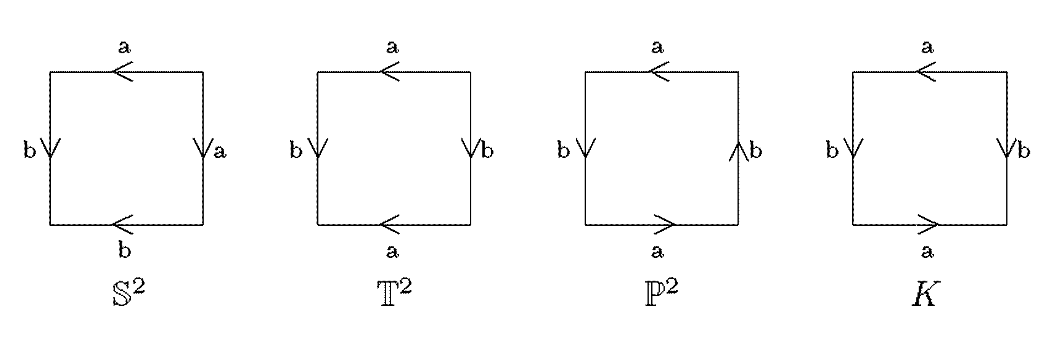
\includegraphics[width=\textwidth]{img/realizacion-geom.png}
\end{center}

El siguiente lema simplifica la demostración del teorema de clasificación, mostrando la equivalencia entre ciertos tipos de superficies.

\lemp{Equivalencia entre algunos tipos de superficies}{
    \label{lem:toro-proyectivo}
    \begin{enumerate}
        \item La botella de Klein y $\mathbb{RP}^2\#\mathbb{RP}^2$ son homeomorfas.
        \item $\mathbb{T}^2\#\mathbb{RP}^2$ y $\mathbb{RP}^2\#\mathbb{RP}^2\#\mathbb{RP}^2$ son homeomorfas.
    \end{enumerate}
}{
    Para la primera parte nos fijamos en el siguiente dibujo:
    \begin{center}
        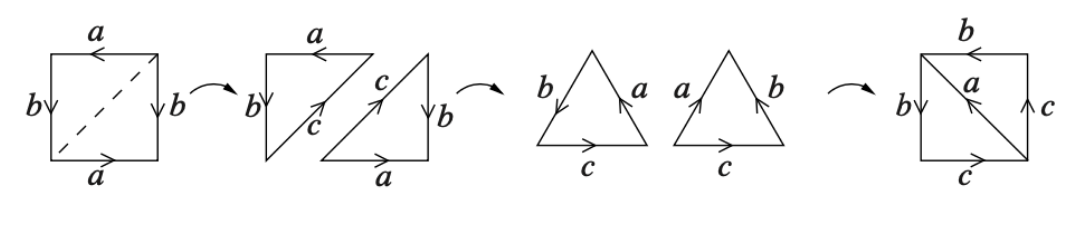
\includegraphics[width=0.8\textwidth]{img/botella-klein-transformacion.png}
    \end{center}
    Por tanto a la presentación de la botella de Klein dada por $\langle a,b\mid abab^{-1} \rangle$ le aplicamos un corte, una reflexión, dos rotaciones, un pegado y una última rotación:
    \begin{align*}
        \langle a,b\mid abab^{-1} \rangle &\cong \langle a,b,c\mid abc, c^{-1}ab^{-1} \rangle \cong \langle a,b,c\mid abc,ba^{-1}c \rangle \\
        &\cong \langle a,b,c\mid bca,a^{-1}cb \rangle \cong \langle b,c\mid bccb \rangle \cong \langle b,c\mid bbcc \rangle
    \end{align*}
    y llegamos a una presentación de la suma conexa de dos proyectivos.

    Para la segunda parte nos fijamos en este otro dibujo:
    \begin{center}
        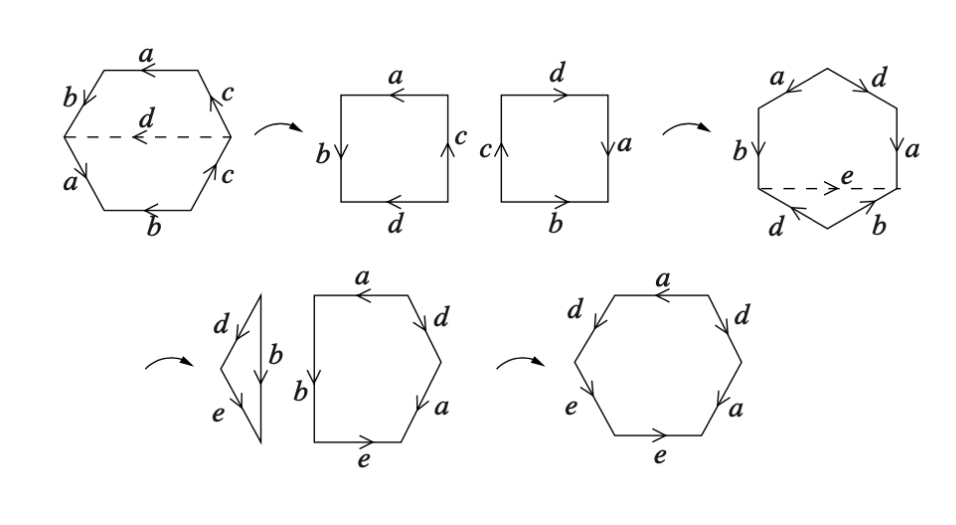
\includegraphics[width=0.6\textwidth]{img/toro-proyectivo-transformacion.png}
    \end{center}
    Partimos de una presentación de $K\#\mathbb{RP}^2$, que por la parte 1 sabemos que es homeomorfo a $\mathbb{RP}^2\#\mathbb{RP}^2\#\mathbb{RP}^2$. La presentación está dada por $\langle a,b\mid abab^{-1}cc \rangle$, y le aplicamos las transformaciones de la figura (ejercicio para el lector: indicar qué transformaciones elementales se usan en cada paso)
    \begin{align*}
        \langle a,b,c\mid abab^{-1}cc \rangle &\cong \langle a,b,c,d\mid abd^{-1}c, c^{-1}ba^{-1}d^{-1} \rangle \cong \langle a,b,d\mid abd^{-1}ba^{-1}d^{-1} \rangle \\
        &\cong \langle a,b,d,e\mid deb^{-1},bea^{-1}d^{-1}a \rangle \cong \langle a,d,e \mid deea^{-1}d^{-1}a \rangle\\
        &\cong \langle a,d,e \mid a^{-1}d^{-1}adee \rangle
    \end{align*}
    y llegamos a una presentación de la suma conexa de un toro y un proyectivo.
}

\thm{Clasificación de superficies compactas}{
    \label{thm:clasificacion-superficies}
    Sea $S$ una superficie compacta y conexa, entonces $S$ es homeomorfa a una de las siguientes superficies:
    \begin{itemize}
        \item la esfera $\mathbb{S}^2$.
        \item una suma conexa de toros $\mathbb{T}^2\#\dots\#\mathbb{T}^2$.
        \item una suma conexa de planos proyectivos $\mathbb{RP}^2\#\dots\#\mathbb{RP}^2$.
    \end{itemize}
}
\pf{
    \noindent
    Sea $M$ una superficie compacta y conexa y sea $\partes$ su presentación poligonal, la cual sabemos que existe por el \hyperref[thm:rado]{Teorema de Radó}.

    \vspace{1em}
    \noindent
    \underline{Objetivo:} aplicar transformaciones elementales a $\partes$ hasta llegar a uno de los siguientes casos:
    \[
        \partes \cong 
        \begin{cases}
            \langle a \vert a a^{-1} \rangle, & \text{presentación de } \mathbb{S}^2, \\[6pt]
            \langle a_1, b_1, \dots, a_n, b_n \vert a_1b_1a_1^{-1}b_1^{-1}\dots a_n b_n a_n^{-1}b_n^{-1} \rangle, 
            & \text{presentación de } \mathbb{T}^2\#\dots\#\mathbb{T}^2, \\[6pt]
            \langle a_1, \dots, a_n \vert a_1a_1\dots a_n a_n \rangle, 
            & \text{presentación de } \mathbb{RP}^2\#\dots\#\mathbb{RP}^2.
        \end{cases}
    \]

    \vspace{1em}
    \noindent
    Para ello, separamos la demostración en 7 pasos, en cada uno de los cuales manipulamos $\partes$ para que cumpla una determinada condición 
    (nótese el abuso de notación al llamar $\partes$ tanto a la presentación original como a la presentación $\partes '$ obtenida tras aplicar una transformación elemental). 
    Al término del último paso, llegaremos a que $\partes$ adopta una de las formas canónicas anteriores.

    \vspace{1em}
    \noindent
    Durante la demostración, llamaremos \emph{aristas complementarias} a aquellas que aparecen en $\partes$ como $a$ y $a^{-1}$, y 
    \emph{aristas retorcidas} a las que aparecen como $a$ y $a$, o $a^{-1}$ y $a^{-1}$.

    \vspace{1.3em}
    \noindent
    \underline{PASO 1:}
    \begin{quote}
        Podemos suponer que $\partes$ tiene solo una palabra (o que el polígono tiene 1 sola cara).
    \end{quote}

    \noindent
    Una consecuencia de que la superficie sea conexa es la siguiente: si $\partes$ tiene varias palabras, para cada palabra debe existir una arista que se identifique con una arista de otra palabra. 
    Es decir, siempre que $\partes$ tenga varias palabras, para cada palabra $W_1$ de $\partes$ debe existir una arista $a \in W_1$ y una palabra $W_2$ tal que 
    o bien $a\in W_2$ o $a^{-1}\in W_2$. En caso de que esto no ocurra, en la realización geométrica $W_1$ y las demás palabras serían disjuntas, formando así una separación que
    contradice la conexión de $M$.

    \vspace{0.5em}
    \noindent
    Ahora, si $W_1$ es una palabra y $\partes$ tiene más de una palabra, por lo anterior existe una arista $a$ que conecta con otra palabra $W_2$ 
    (ya sea mediante $a$ o $a^{-1}$). Pegando $W_1$ y $W_2$ (aplicando rotaciones y reflejos si fuera necesario), 
    obtenemos una presentación donde $W_1$ y $W_2$ se han sustituido por una única nueva palabra $W_1'W_2'$. 

    \vspace{0.5em}
    \noindent
    Como el número de palabras de la presentación original es finito, mediante este proceso se obtiene una presentación equivalente compuesta por una sola palabra.

    \vspace{1.3em}
    \noindent
    \underline{PASO 2:}
    \begin{quote}
        Podemos suponer que no hay pares de aristas complementarias adyacentes ($W_1aa^{-1}W_2$).
    \end{quote}

    \noindent
    Si las hubiera, plegando por ellas desaparecen. Excepto el caso en que solo tengamos ese par ($W_1, W_2 = \emptyset$). 
    Pero entonces la superficie es una esfera, que es una de las formas canónicas que pretendíamos obtener.

    \vspace{1.3em}
    \noindent
    \underline{PASO 3:}
    \begin{quote}
        Podemos suponer que todos los pares de aristas retorcidas son adyacentes.
    \end{quote}

    \noindent
    Supongamos que tenemos $VaWa$, con $V,W \ne \emptyset$. Cortamos por el medio ($Vab$ y $b^{-1}Wa$). 
    Rotamos y reflejamos la segunda palabra ($bVa$ y $a^{-1}W^{-1}b$), y pegamos por $a$ llegando a $bbVW^{-1}$, donde las aristas retorcidas ya son adyacentes. 
    La repetición de este proceso una cantidad finita de veces demuestra el paso 3.
    
    \begin{center}
        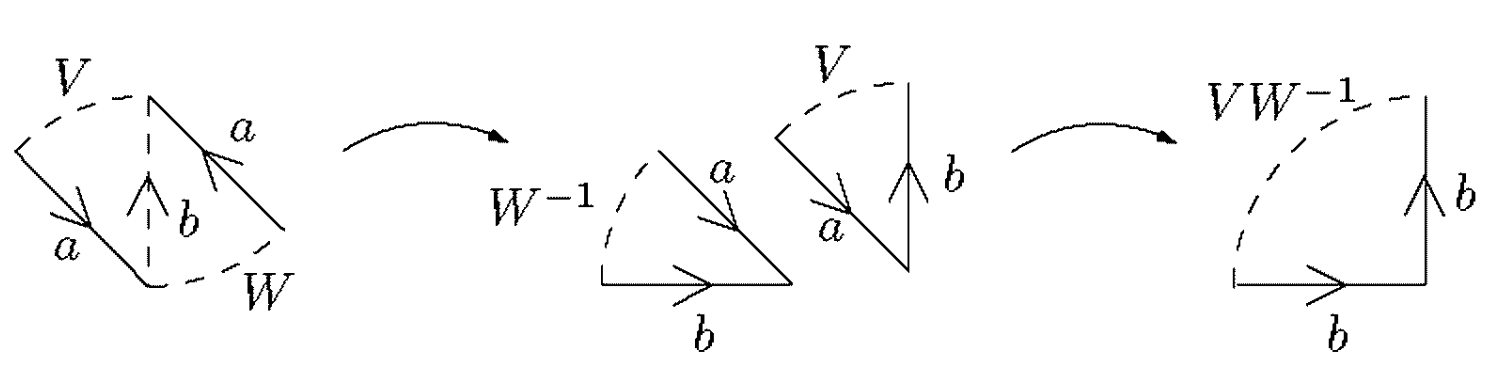
\includegraphics[width=0.6\textwidth]{img/teorema-clasificacion/paso3.png}
    \end{center}

    \noindent
    \textit{Nota:} En cada iteración, es posible que tengamos que volver a aplicar el paso 2 ya que al pegar $V$ y $W^{-1}$ en $VW^{-1}$ podrían aparecer nuevas aristas complementarias adyacentes.

    \vspace{1.3em}
    \noindent
    \underline{PASO 4:}
    \begin{quote}
        Podemos suponer que el polígono tiene todos sus vértices identificados.
    \end{quote}

    \noindent
    Sea $p:\partes \to M$ la proyección al cociente. Sea $p(v)=[v]$. 
    Si no todos los vértices están identificados, existen vértices $v_1, w$ en $\partes$ 
    y una arista $ a : v_1 \to w$ con $p(v_1)\ne p(w)$. 
    Ahora, la arista que termina en $v_1$ no puede ser ni $a$ (porque entonces $p(v_1) = p(w)$) 
    ni $a^{-1}$ (pues tendríamos la secuencia $a^{-1} a$ y al aplicar de nuevo el paso 2 llegaríamos también a que $p(v_1) = p(w)$). 
    Por tanto, concluimos que la arista es distinta, llamémosla $b$, y al vértice del que parte $x$. 
    Es decir, tenemos $b : x \to v_1$.

    \vspace{0.5em}
    \noindent
    Por la definición de presentación poligonal, la letra $b$ debe aparecer (bien como $b$ o como $b^{-1}$) en otro sitio de la presentación. 
    Suponemos que aparece $b^{-1}$ (si fuese $b$ sería análogo salvo una reflexión que ahora mencionaremos). 
    Tenemos entonces por construcción la secuencia $baXb^{-1}Y$, con $X$ e $Y$ cadenas arbitrarias de la presentación. Podemos suponer $X,Y \ne \emptyset$. Veámos por qué:
    \begin{itemize}
        \item Si $X$ fuese vacío, por la definición de $b$, el vértice al que llega $b^{-1}$ en nuestra cadena no sería otro que $w$ (recordemos $a:v_1\to w$). 
              Pero entonces $p(v_1) = p(w)$, lo que contradice la hipótesis.
        \item Si $Y$ fuese vacío, rotando obtendríamos dos aristas adyacentes $b$ y $b^{-1}$ y estaríamos en el paso 2.
    \end{itemize}

    \vspace{0.5em}
    \noindent
    Ahora, cortando por una nueva arista $c : w \to x$, rotando para pegar por $b$ 
    (y reflejando si en vez de tener $b^{-1}$ tuviéramos $b$) obtenemos:
    \[
        baXb^{-1}Y \;\cong\; bac \text{, } c^{-1}Xb^{-1}Y \;\cong\; acb \text{, } b^{-1}Yc^{-1}X \;\cong\; acYc^{-1}X
    \]

    \begin{center}
        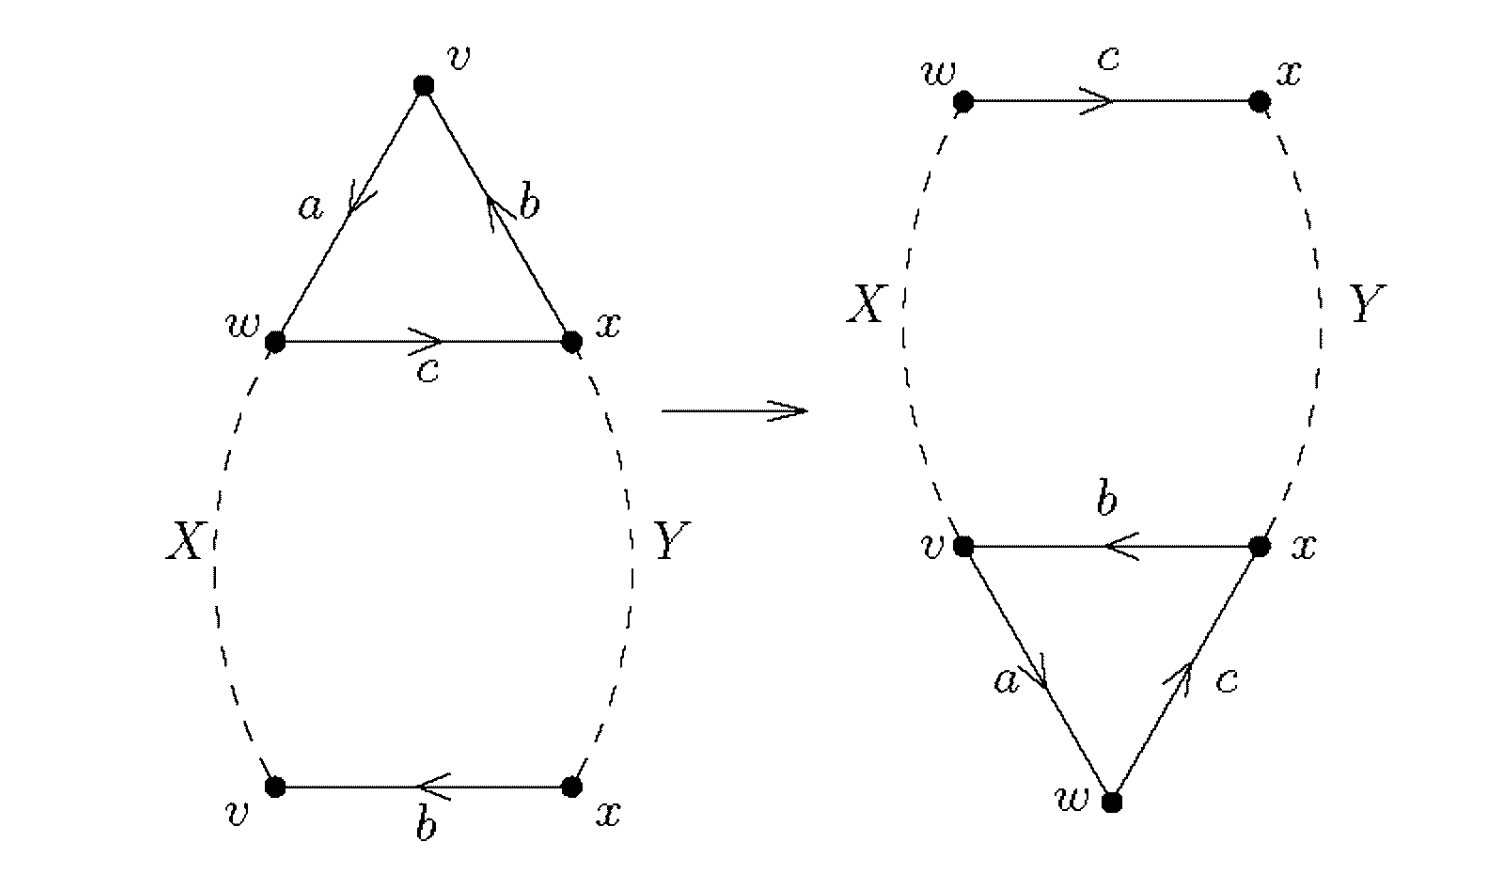
\includegraphics[width=0.6\textwidth]{img/teorema-clasificacion/paso4.png}
    \end{center}

    \noindent
    Incluyendo los vértices en la presentación a la que hemos llegado, 
    \[
        v_1 \overset{a}{\to} w \overset{c}{\to} x \overset{Y}{\to} x \overset{c^{-1}}{\to} w \overset{X}{\to} v_1
    \]
    que es una presentación equivalente donde hemos reducido la cantidad de vértices que se identifican con $v_1$ en una unidad.

    \vspace{0.5em}
    \noindent
    \textit{Nota:} De nuevo, podría ser que al pegar $X a$ aparecieran nuevas aristas complementarias adyacentes. 
    En ese caso, se aplicaría el paso 2, donde en ningún caso se pueden aumentar los vértices identificados con $v_1$, solo disminuirlos.

    \vspace{0.5em}
    \noindent
    Una cantidad finita de iteraciones de este proceso elimina la clase de equivalencia de vértices $v_1$, 
    pues en cada paso se elimina un elemento de este conjunto finito. 
    Repitiendo para cada clase de equivalencia de vértices, llegamos a que solo puede quedar una, 
    demostrando así el paso 4.

    \vspace{1.3em}
    \noindent
    \underline{PASO 5:}
    \begin{quote}
        Se cumple que si aparece un par $a, a^{-1}$, entonces hay otro par $b, b^{-1}$ intercalado, 
        es decir, de la forma $a\dots b\dots a^{-1} \dots b^{-1}$.
    \end{quote}

    \noindent
    Si no fuese así, tendríamos una presentación de la forma $aXa^{-1}Y$, donde además $X$ e $Y$ no comparten aristas 
    (si compartiesen alguna letra $b$, por hipótesis ésta debería aparecer como $b$, y no como $b^{-1}$, tanto en $X$ como en $Y$, 
    lo cual no es posible por el paso 3). 
    Esto significa también que $X$ e $Y$ no comparten vértices, ya que si $x$ fuese un vértice de $X$ y $y$ un vértice de $Y$ tales que acaban identificados en la proyección,
    por cómo se define la relación de equivalencia tendría que haber una arista a la vez en $X$ y en $Y$, contradiciendo así que $X$ e $Y$ no comparten aristas.

    \begin{center}
        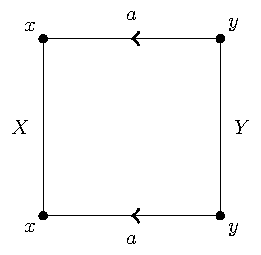
\includegraphics[width=0.3\textwidth]{img/teorema-clasificacion/paso5.pdf}
    \end{center}

    \vspace{0.5em}
    \noindent
    En particular, los vértices finales de $a$ y $a^{-1}$, que están ambos en $X$, 
    solo pueden identificarse con vértices de $X$. 
    Por otro lado, los vértices iniciales de $a$ y $a^{-1}$, que están ambos en $Y$, 
    solo pueden identificarse con vértices de $Y$. 
    Entonces, existen dos clases de equivalencia de vértices distintas, 
    lo que contradice el paso 4. Por tanto no puede darse la situación $aXa^{-1}Y$ y los pares de aristas retorcidas deben estar intercalados.

    \vspace{1.3em}
    \noindent
    \underline{PASO 6:}
    \begin{quote}
        Podemos suponer que los pares de aristas del paso 5 aparecen consecutivos.
    \end{quote}

    \noindent
    Tenemos ahora una cadena $aXbYa^{-1}Zb^{-1}W$, 
    y buscamos hacer transformaciones para que las aristas aparezcan consecutivas. 
    Empezamos con nuestra presentación original, la cual rotamos para cortar desde el final de $X$ al final de $W$, llamando a la arista del corte $c$. 
    \[
        aXbYa^{-1}Zb^{-1}W \cong WaXbYa^{-1}Zb^{-1} \;\;\cong\;\; WaXc \text{, } c^{-1}bYa^{-1}Zb^{-1}
    \]
    \noindent 
    Vamos a pegar por $a$, para lo cual tenemos primero que rotar.
    \[
        WaXc \text{, } c^{-1}bYa^{-1}Zb^{-1} \cong XcWa \text{, } a^{-1}Zb^{-1}c^{-1}bY \;\;\cong\;\; XcWZb^{-1}c^{-1}bY
    \] 
    \noindent
    Ahora cortamos desde el final de $b^{-1}$ al final de $c$, llamando $d$ a esa arista. 
    \[
        XcWZb^{-1}c^{-1}bY \;\;\cong\;\; c^{-1}bYXcWZb^{-1} \;\;\cong\;\; c^{-1}bYXcd \text{, } d^{-1}WZb^{-1}
    \]

    \noindent
    Por último, rotando y pegando por $b$ conseguimos que las cuatro aristas queden consecutivas.
    \[
        c^{-1}bYXcd \text{, } d^{-1}WZb^{-1} \cong YXcdc^{-1}b \text{, } b^{-1}d^{-1}WZ \;\;\cong\;\; YXcdc^{-1}d^{-1}WZ
    \]

    \begin{center}
        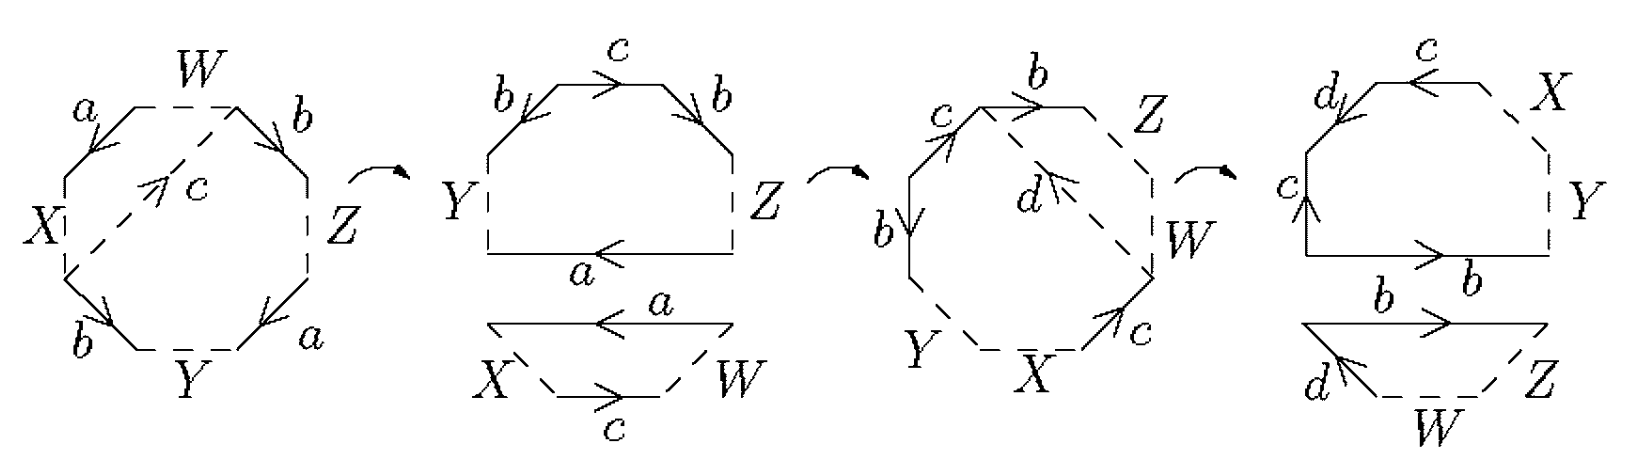
\includegraphics[width=0.7\textwidth]{img/teorema-clasificacion/paso6.png}
    \end{center}

    \vspace{0.5em}
    \noindent
    Haciendo esto para todos los pares de aristas intercalados que no sean consecutivos se demuestra el paso 6.

    \vspace{1.3em}
    \noindent
    \underline{PASO 7:}
    \begin{quote}
        La superficie $M$ es homeomorfa a $\mathbb{T}^2\#\dots\#\mathbb{T}^2$, o bien a $\mathbb{RP}^2\#\dots\#\mathbb{RP}^2$.
    \end{quote}

    \noindent
    Con todo lo que hemos hecho hasta ahora, nuestra presentación solo puede contener los siguientes tipos de elementos:

    \begin{enumerate}
        \item Parejas de aristas complementarias consecutivas, de la forma $aba^{-1}b^{-1}$.
        \item Aristas retorcidas de la forma $aa$.
    \end{enumerate}

    \noindent
    Recordemos que la presentación poligonal de un toro viene dada precisamente por la forma $a b a^{-1} b^{-1}$, 
    y la presentación de un plano proyectivo por $aa$. 
    Por tanto, si solo hubiese aristas de una de estas dos formas, 
    la superficie sería homeomorfa a una suma conexa de toros o de planos proyectivos, respectivamente.

    \vspace{0.5em}
    \noindent
    Nos queda ver qué ocurre en el caso de que $\partes$ contenga ambos grupos de aristas. 
    Supongamos que existen un grupo de aristas complementarias $aba^{-1}b^{-1}$ y otro de aristas retorcidas $cc$. 
    Por el lema \hyperref[lem:toro-proyectivo]{2.6.1}, la suma conexa de un toro y un plano proyectivo es homeomorfa a la suma conexa de tres planos proyectivos. 
    Es decir, $aba^{-1}b^{-1}cc \cong a'a'b'b'c'c'$. 
    Transformando cada par (toro, proyectivo) en tres proyectivos podemos eliminar los toros y quedarnos con un número finito de planos proyectivos.

    \vspace{0.5em}
    \noindent
    Concluyendo, si $\partes$ tiene solo aristas complementarias alternadas, es homeomorfa a una suma conexa de toros. 
    Si tiene solo aristas retorcidas, es homeomorfa a una suma conexa de planos proyectivos. 
    Y si tiene ambos tipos de aristas, es homeomorfa a una suma de planos proyectivos.
}

\propp{Característica de Euler invariante por transformaciones elementales}{
    La característica de Euler de una presentación poligonal es invariante por transformaciones elementales
}{
    Es inmediato que al renombrar, reflejar y rotar no cambiamos el número de vértices, aristas y caras, por lo que $\chi$ no cambia. Para el resto de transformaciones veamos que los cambios en $F,E,V$ se <<compensan>>:
    \begin{itemize}
    \item Consolidar y dividir
    \[ \text{3 vertices, 2 aristas $\longleftrightarrow$ 2 vértices, 1 arista, $\chi$ se mantiene.} \]

    \item Cortar y pegar
    \[\text{1 cara, 2 aristas $\longleftrightarrow$ 2 caras, 3 aristas, $\chi$ se mantiene.}\]

    \item Plegar y desplegar:
    \[\text{1 vértice $\longleftrightarrow$ 2 vértices, 1 arista, $\chi$ se mantiene.}\]
    \end{itemize}
}

\defn{Característica de Euler de una superficie compacta}{
    Dada una superficie compacta $M$, se define su característica de Euler $\chi(M)$ como la característica de cualquier presentación poligonal de ella (ya que es invariante por transformaciones elementales).
}

\ex{
    Característica de Euler en las superficies modelo (recordando sus representaciones <<estándar>>):
    \begin{enumerate}
        \item $\chi(\mathbb{S}^2) = 1-1+2 = 2$.
        \item $\chi(n\mathbb{T}^2) = 1-2n+1 = 2-2n$.
        \item $\chi(n\mathbb{RP}^2) = 1-n+1 = 2-n$.
    \end{enumerate}
}

\rmkb{
    Para todo poliedro de $\R^3$, esto es, un sólido bordeado por un conjunto finito de polígonos convexos unidos por los lados, que sea homeomorfo a la esfera $\mathbb{S}^2$ se tiene que
    \[ \chi = V - E + F = 2 \]
}

\section{Orientabilidad}

\defn{Superficie orientable}{
    Una superficie compacta se dice orientable si admite una presentación poligonal en la que no existe ningún par de aristas que se identifiquen recorriéndose en el mismo sentido, es decir, si para cada arista $a$ de la presentación, aparece tanto $a$ como $a^{-1}$.
}

\propp{}{
    Una superficie compacta no orientable contiene un subespacio homeomorfo a la cinta de Möbius (de hecho es un si y solo si).
}{
    \noindent ($\implies$) Siempre tenemos aristas identificadas $aa$.
    Demostración con dibujitos, no puedo hacerlo :(
    
    \noindent ($\impliedby$) Sea una presentación:
    
    \noindent\underline{Afirmación 1:} El subespacio homeomorfo a la cinta de Möbius toca al borde. No entra en detalle, si alguien quiere hacerlo que se las apañe jeje.
}

\ex{
    \noindent Superficies no orientables: $\mathbb{RP}^2$, $K$ (la botella).
    
    \noindent Superficies orientables: $\mathbb{S}^2$, $\mathbb{T}^2$.
}

\propp{Orientabilidad de la suma conexa}{
    Dadas dos superficies compactas $S_1$ y $S_2$, la suma conexa $S_1\# S_2$ es orientable si, y solo si, ambas superficies son orientables.
}{
    Pendiente...
}

\ex{
    $\mathbb{T}^2 \# \dots \# \mathbb{T}^2$ es orientable.
    $\mathbb{RP}^2 \# \dots \# \mathbb{RP}^2$ es no orientable.
}

\corp{
    Dos superficies compactas y conexas son homeomorfas si, y solo si, tienen la misma característica de Euler y la misma orientabilidad.
}{
    Pendiente...
}

\defn{Género de una superficie}{
    Sea $S$ una superficie compacta y conexa. Se define el género de $S$ como $g(S) = 1-\frac{1}{2}\chi(S)$ si $S$ es orientable, y $g(S) = 2 - \chi(S)$ si no lo es. El género también se conoce como el número de agujeros.
}

\ex{
    \begin{itemize}
        \item $g(\mathbb{S}^2) = 0 = g(0\mathbb{T})$.
        \item $g(\mathbb{T}^2 \# \dots \# \mathbb{T}^2) = n$.
        \item $g(\mathbb{RP}^2 \# \dots \# \mathbb{RP}^2) = n$.
    \end{itemize}
}

\corp{
    Si $S$ es una superficie compacta, conexa y orientable, entonces $S$ es homeomorfa a:
    \[\begin{cases}
        \text{una esfera, cuando $g(S) = 0$} \\
        \text{una suma conexa de $n$ toros, cuando $g(S) = n, n \ge 1$}
    \end{cases}\]
}{
    Sea $S$ una superficie compacta, conexa y orientable. Por definición, existe una presentación $\mathcal{P}$ que no tiene pares de aristas retorcidas. Además, por el \hyperref[thm:clasificacion-superficies]{Teorema de Clasificación}, $S$ debe ser homeomorfa a una suma conexa de una de las tres superficies modelo. Basta ver que a partir de la presentación $\mathcal{P}$ no se puede llegar a una suma conexa de planos proyectivos. 

    Nótese que en una presentación sin pares de aristas retorcidas, la única forma de que aparezcan mediante transformaciones es cortando y haciendo un reflejo en una de las palabras. Seguimos el algoritmo de la demostración del \hyperref[thm:clasificacion-superficies]{Teorema de Clasificación}, teniendo como hipótesis que en $\mathcal{P}$ inicialmente no hay aristas retorcidas, para observar que nunca aplicamos reflejos y por tanto no llegamos a un plano proyectivo (recomendamos tener dicha demostración delante para ver esta, pues son comentarios a los pasos de la misma).

    \begin{enumerate}
        \item Si $\mathcal{P}$ tiene más de una palabra, para pegar solo hay que hacer rotaciones y no reflejos (pues todos los pares ya son de la forma $a, a^{-1}$).
        \item No se hacen reflejos en ningún caso.
        \item No hay aristas retorcidas, así que el paso no se aplica.
        \item Recordemos la construcción $ a: v_1\to w$, $b: x \to v_1$. La otra aparición de $b$ en la presentación debe ser como $b^{-1}$, y por tanto no es necesario aplicar ninguna reflexión.
        \item No se aplican reflejos.
        \item Ninguna transformación de las que se hacen es un reflejo.
        \item Una vez llegamos a este paso, podemos concluir directamente que estamos ante una suma de toros, pues sabemos que no hay ningún par de aristas retorcidas. 
    \end{enumerate}
}